% Self-created synthetic vector figure. No real research claims or measurements.
% Build with the same pdfLaTeX toolchain as the gallery; no extra packages.
\documentclass{article}
\usepackage{tikz}
\usetikzlibrary{arrows.meta}
\pagestyle{empty}
\setlength{\paperwidth}{420pt}
\setlength{\paperheight}{168pt}
\setlength{\textwidth}{420pt}
\setlength{\textheight}{168pt}
\setlength{\oddsidemargin}{-1in}
\setlength{\topmargin}{-1in}
\setlength{\headheight}{0pt}
\setlength{\headsep}{0pt}
\setlength{\topskip}{0pt}
\setlength{\parindent}{0pt}
\pdfpagewidth=420pt
\pdfpageheight=168pt
\definecolor{FigurePurple}{HTML}{6E438D}
\definecolor{FigureOrange}{HTML}{C67B19}
\begin{document}
\noindent\begin{tikzpicture}[x=28pt,y=28pt,>=Stealth,
  font=\sffamily\fontsize{12}{14}\selectfont,
  box/.style={draw=FigurePurple,fill=FigurePurple!10,rounded corners,
    minimum height=30pt,align=center}]
  \path[use as bounding box] (0,0) rectangle (15,5.8);
  \node[font=\sffamily\bfseries] at (2,5.15) {(a) Propose};
  \node[font=\sffamily\bfseries] at (7.5,5.15) {(b) Check};
  \node[font=\sffamily\bfseries] at (12.8,5.15) {(c) Retain};
  \draw[gray,densely dotted] (4.2,1.2) rectangle (10.6,4.65);
  \node[box,minimum width=80pt] (candidate) at (2,3.3) {Candidate $h$};
  \node[box,minimum width=62pt] (evaluate) at (5.8,3.3) {Evaluate $h$};
  \node[box,minimum width=62pt,draw=FigureOrange,fill=FigureOrange!12]
    (accept) at (9.3,3.3) {Accept?};
  \node[box,minimum width=78pt] (retained) at (12.8,3.3) {Retained $h^*$};
  \draw[->,thick,FigurePurple] (candidate)--(evaluate);
  \draw[->,thick,FigurePurple] (evaluate)--node[above]{score} (accept);
  \draw[->,thick,FigurePurple] (accept)--node[above,pos=0.35]{yes} (retained);
  \draw[->,thick,dashed,FigureOrange] (accept.south)--(9.3,1.9)
    --node[below]{no: revise} (2,1.9)--(candidate.south);
  \draw[->,thick,FigurePurple] (0.7,0.65)--(1.7,0.65);
  \node[anchor=west] at (1.9,0.65) {forward flow};
  \draw[->,thick,dashed,FigureOrange] (7.2,0.65)--(8.2,0.65);
  \node[anchor=west] at (8.4,0.65) {revision feedback};
\end{tikzpicture}
\end{document}
